\chapter{Cotas comunes}

Retomamos el problema de admisión a universidades igual que como se plantea en el capítulo 4, se agrega la restricción de que varias universidades en conjunto pueden compartir cotas superiores, estas restricciones son de carácter natural porque las universidades pueden tener recursos compartidos como es el caso, por ejemplo, de becas gubernamentales . En particular se le agregan la siguiente restricción al problema:


%Para abreviar llamaremos a este problema \textbf{CA-CQ}.
\begin{equation}
\sum_{i=1}^{n} \sum_{j=1}^m w_{j,k} \cdot x_{i,j} \leq N_k %\cdot z_k
\end{equation} 
donde \begin{equation} w_{j,k}= 
\begin{cases}
1 & \qquad \text{si la universidad $j$ es parte de la restricción $k$.} \\
0 &\qquad\text{en otro caso.} \\ 
\end{cases} \end{equation} \\ para toda $k=1,2,\dots,p$ \footnote{Donde $p$ es el número de restricciones comunes.}. \\
Las universidades tienen cotas superiores comunes.
%\item \begin{equation} 
%z_{k}= 
%\begin{cases}
%1 & \qquad \text{si las universidades en la restricción $k$ abren.} \\
%0 &\qquad\text{en otro caso.}\ \\ 
%\end{cases} \end{equation}

%\item \begin{equation}
%\sum_{j=1}^{m} w_{j,k} y_{j} \leq z_{k} \text{ para toda $k=1,2,\dots,p$. }
%\end{equation} \\ Las universidades solo pueden abrir si cumplen su cota común. 

%\item \begin{equation} \label{r6}
%x_{i,j} \leq y_j \ \text{ para toda $i=1,2,\ldots,n$ y para toda $j=1,2,\ldots,m$.}
%\end{equation}
%Los solicitantes únicamente pueden asistir a universidades abiertas.


Para simplificar la notación del problema, en lugar de usar la matriz de preferencias definida por \ref{matpref} utilizaremos una lista de preferencias que tiene la ventaja de ser un poco más simple para expresar las cotas comunes. 

\begin{dfn}
\label{listpref}
Definimos la \textbf{lista de preferencias} para un problema con $n$ estudiantes, con $m$ universidades y $p$ restricciones
como una función $P$ de tal forma que si $\alpha$ es un estudiante $P(\alpha)$ es el orden de preferencia que le asigna a las universidades,
si $A$ es una universidad $P(A)$ es el orden de preferencia que le asigna a los estudiantes, salvo que el primer lugar denota la cota superior de $A$.
Además, si denotamos a $\mathcal{C}$ como el \textbf{sistema de conjuntos de universidades} %(ver \ref{conj1})
que está conformado por los conjuntos de universidades que forman cada restricción y denotamos $C_k$ como el conjunto de universidades que forman parte de la restricción común $k$ para todo $k=1,2,\dots,p$;
Entonces $P(C_k)$ representa el orden de preferencias de la cota $C_k$ para todo $k=1,2,\dots,p$.

Es un poco contraintuitivo definir las preferencias en términos de conjuntos de universidades, esto es necesario, por ejemplo, en situaciones cuando se alcanza la cota común entre dos universidades, pero ninguna alcanza su cota superior. Si sólo nos basamos en las listas de preferencia de las dos universidades no es claro bajo qué criterio se aceptan o se rechazan nuevos estudiantes. Además, para que exista consistencia en los órdenes de preferencias hacemos los siguientes supuestos:
\begin{enumerate}
\item Si para alguna $k=1,2,\dots,p$ fija, existe una universidad $A$ que pertenece a $C_k$ y además existe un estudiante $\alpha$ que pertenece a $P(A)$. Entonces, $\alpha$ pertenece a $P(C_k)$.
\item Si para alguna $k=1,2,\dots,p$ fija, existe un estudiante $\alpha$ que pertenece a $P(C_k)$, entonces, existe una universidad $A$ que pertenece a $C_k$ tal que $\alpha$ pertenece a $P(A)$.
\item Si para alguna $k=1,2,\dots,p$ fija, existe una universidad $A$ que pertenece a $C_K$ y además existen dos estudiantes $\alpha$ y $\beta$ de tal forma que $A$ prefiere a $\alpha$ sobre $\beta$. Entonces, $\alpha$ aparece antes que $\beta$ en $P(C_K)$.
\item Si para alguna $k=1,2,\dots,p$ fija, existen dos estudiantes $\alpha$ y $\beta$, de tal forma que $\alpha$ aparece antes que $\beta$ en $P(C_k)$. Entonces, toda universidad $A$ que pertenece a $C_k$ prefiere tener a $\alpha$ que a $\beta$ en caso de que aparezcan en $P(A)$.
\end{enumerate}
\end{dfn}

Damos un ejemplo de una lista de preferencias para dejar todo un poco más claro, en general la idea es la misma que las matrices de preferencias.


\begin{eje} \cite{Todo}
\label{listprefeje}
Supongamos que tenemos tres solicitantes $\alpha,\beta, \gamma$, cuatro universidades $A,B,C,D$ y dos conjuntos de universidades $\{A,B\},\{A,C\}$ que forman cotas comunes. La lista de preferencias sigue la siguiente regla:

\noindent \begin{minipage}{.3\linewidth}
$$P(\alpha)=A,D$$ \\
$$P(\beta)=B$$ \\
$$P(\gamma)=D,C$$ 
\end{minipage}%
\begin{minipage}{.3\linewidth}
$$P(A)=1:\alpha$$ \\
$$P(B)=1:\beta$$ \\
$$P(C)=1: \gamma$$ \\
$$P(D)=1: \alpha, \gamma$$ 
\end{minipage}
\begin{minipage}{.4\linewidth}
$$P(\{A,B\})= 1:\beta,\alpha$$ \\
$$P(\{A,C\})=1:\gamma,\beta$$
\end{minipage}
\medskip

Aquí (solo para dar algunos ejemplos) podemos ver que $\alpha$ tiene en su lista primero a $A$ y luego a $D$. $C$ únicamente quiere a $\gamma$ como su alumno y además tiene como cota superior al número uno. Las cotas comunes son consistentes de acuerdo con lo planteado anteriormente. 
\fin
\end{eje}

La primera pregunta que uno podría hacerse es si siempre existe una asignación estable. Recordemos que en el caso de cotas inferiores no siempre existe y por lo tanto podría aquí suceder lo mismo. El siguiente resultado muestra que de hecho no siempre existe una asignación estable para el problema.

\begin{teo} \cite{Todo}
\label{ejemplo teorema}
Dada una instancia del problema de admisión a universidades con cotas comunes podría no existir solución al problema de encontrar una asignación estable.
\end{teo}
\begin{proof}
Supongamos que para lista \ref{listprefeje} existe una asignación estable $M$. Si $\alpha$ no está emparejada llegamos a una contradicción porque $D$ tiene a $\alpha$ primero en su lista y no está bloqueada por ninguna restricción común. es decir, no existe razón para que $\alpha$ no esté asignada. 

Si $\alpha$ esta asignada a $A$ tenemos que entonces $\gamma$ esta asignada a $D$ y además por la restricción común de $\{A,B\}$, $\beta$ queda sin estar asignado lo cual contradice la hipótesis de estabilidad porque $\{A,B\}$ prefiere tener a $\beta$ que a $\alpha$. 

Si $\alpha$ este asignado a $D$ entonces $\gamma$ está asignado a $C$ lo que implica que $\beta$ queda sin estar asignado. $\{A,B\}$ y $A$ no cumplen con su cota superior (tienen espacio para más alumnos) y $\alpha$ prefiere estar en $A$ que en $D$, por lo tanto, esta asignación no es estable y de hecho concluimos que no existen asignaciones estables para este problema. 

Notamos que si $\beta$ no fuera parte del problema entonces si asignamos $\alpha$ a $A$ y asignamos $\gamma$ a $D$ tenemos una asignación estable, por lo tanto, concluimos que a veces sí existe una asignación estable. 
\end{proof}

%Además de no siempre existir una asignación estable sucede algo muy similar a lo planteado en el capítulo 5, en el que podría existir varios emparejamientos estables para el mismo problema de distinto tamaño. El siguiente ejemplo muestra que para este problema también sucede lo mismo.

A partir de este ejemplo queda claro que si extendemos el problema agregando cotas comunes perdemos la garantía de existencia de un emparejamiento estable en nuestro problema. La pregunta clave aquí es si existe alguna condición que garantice la existencia de un emparejamiento estable para cualquier problema de este tipo o si existe algún algoritmo para llegar a uno de forma eficiente, el siguiente resultado muestra que esta pregunta es mucho más complicada de lo que parece. 

\begin{teo} \cite{Todo}
El problema de ver si una instancia del problema de admisión a universidades con cotas comunes admite un emparejamiento estable es NP-completo. 
\end{teo}
\begin{proof}
\footnote{La demostración se parece bastante a la del teorema \ref{np1}.}
Dado que el problema claramente es de decisión y además dada una solución es fácil ver si ésta es correcta o no, éste pertenece a la clase NP.

Para ver que el problema es NP-completo reduciremos el problema del matrimonio estable con listas incompletas con empates a éste\footnote{Recordemos que el problema aquí es ver si existe un emparejamiento estable con todos los hombres y todas las mujeres emparejadas.} (sabemos que este problema es NP-completo por el teorema \ref{NPempates}). Para este caso supondremos que sólo existen empates en las listas de las mujeres, estos son de a lo más longitud 2 y en caso de existir un empate para una mujer arbitraria $w_j$, éste ocupa toda la lista de $w_j$ y al menos uno de los dos hombres pertenecientes a esté tiene a $w_j$ hasta arriba de su lista\footnote{Dadas estas condiciones el problema sigue siendo NP-completo \cite{empates}}. 

Sea $I$ una instancia del problema del emparejamiento estable con listas incompletas con empates, sean $U=\{m_1,m_2,\dots,m_n\}$ la lista de hombres en el problema y sean $W=\{w_1,w_2,\dots,w_n\}$ las mujeres en el problema. Sea $W_0$ un subconjunto de $W$ que contiene a todas las mujeres con un empate de tamaño dos en su lista. Construiremos una instancia $I'$ del problema de admisión a universidades con cotas comunes a partir de $I$. 

Cada hombre en $I$ corresponde a un solicitante en $I'$ y sus listas de preferencia son idénticas en ambas instancias. Si las mujeres pertenecen a $W \setminus W_0$ entonces representan a una universidad en $I'$ y cuentan con una cota superior igual al número 1, sus listas de preferencia son idénticas en $I$ y en $I'$. 

El truco está con las mujeres en $W_0$, supongamos que tenemos una mujer $w_j$ en $W_0$ y supongamos que $m_{j,1}$ y $m_{j,2}$ son los dos hombres que conforman este empate. Creamos entonces dos solicitantes adicionales $b_j^1,b_j^2$, seis universidades $c_j^1,c_j^2,c_j^3,c_j^4,c_j^5,c_j^6$ y cuatro conjuntos de universidades $\{c_j^1,c_j^2\},\{c_j^2,c_j^3\},\{c_j^4,c_j^5\},\{c_j^5,c_j^6\}$ con cotas comunes y las siguientes preferencias: 

\begin{minipage}{.3\linewidth}
$$P(b_j^1)=c_j^5,c_j^2$$ \\
$$P(b_j^2)=c_j^3,c_j^6$$ 
\end{minipage}%
\begin{minipage}{.3\linewidth}
$$P(c_j^1)=1:m_{j,1}$$ \\
$$P(c_j^2)=1:b_j^1$$ \\
$$P(c_j^3)=1: b_j^2$$ \\
$$P(c_j^4)=1: m_{j,2}$$ \\
$$P(c_j^5)=1: b_j^1$$ \\
$$P(c_j^6)=1: b_j^2$$ 
\end{minipage}
\begin{minipage}{.4\linewidth}
$$P(\{c_j^1,c_j^2\})= 1:b_j^1,m_{j,1}$$ \\
$$P(\{c_j^2,c_j^3\})=1:b_j^1,b_j^2$$ \\
$$P(\{c_j^4,c_j^5\})= 1:b_j^1,m_{j,2}$$ \\
$$P(\{c_j^5,c_j^6\})=1:b_j^2,b_j^1$$
\end{minipage}

\medskip

Para simplificar la notación, sea $A_1$ los aplicantes de la forma $m_{j,k}$ y sea $A_2$ los aplicantes de la forma $b_j^k$. Finalmente, sustituimos a $w_j$ en la lista de $m_{j,1}$ por $c_{j,1}$ y sustituimos a $w_j$ en la lista de $m_{j,2}$ por $c_{j,4}$. Afirmamos que $I$ tiene un emparejamiento estable completo $M$ si y sólo si $I'$ tiene una asignación estable $M'$ en la que cada solicitante en $A_1$ está asignado a alguna universidad. Suponiendo que en $M$ tenemos que $m_i$ y $w_j$ están emparejados, la relación entre las dos instancias sigue las siguientes reglas:
\begin{itemize}
\item Si $w_j$ pertenece a $W \setminus W_0$, entonces $m_i$ está asignado a $w_j$ en $M'$.
\item Si $w_j$ pertenece a $W_0$, entonces $m_{j,1}$ está emparejado con $w_j$ si y sólo si en $M'$ tenemos que $m_{j,1}$ está asignado a $c_j^1$, $b_j^2$ está asignado a $c_j^3$ y $b_j^1$ está asignado a $c_j^5$.
\item Si $w_j$ pertenece a $W_0$, entonces $m_{j,2}$ está emparejado con $w_j$ si y sólo si en $M'$ tenemos que $m_{j,2}$ está asignado a $c_j^4$, $b_j^2$ está asignado a $c_j^6$ y $b_j^1$ está asignado a $c_j^2$.
\end{itemize}

Supongamos que existe un emparejamiento estable $M$ en $I$, es claro por construcción que la asignación $M'$ resultante es también estable y que además cada solicitante en $A_1$ es asignado a alguna universidad. 

Supongamos que existe una asignación estable $M'$ en $I'$ en el que todos los solicitantes en $A_1$ están emparejados.
% Me falta el párrafo que empieza in the other ddirection.


Para completar la reducción, es necesario construir una parte adicional de $I'$ como sigue: Para cada solicitante $a_i$ en $A_1$ construimos dos solicitantes adicionales $z_i^1,z_i^2$, cuatro universidades $d_i^1,d_i^2,d_i^3,d_i^4$ con cotas comunes $\{d_i^1,d_i^2\}$ y $\{d_i^2,d_i^3\}$. Las listas de preferencias y cotas son como siguen:
\noindent \begin{minipage}{.3\linewidth}
$$P(z_i^1)=d_i^1,d_i^4$$ \\
$$P(z_i^2)=d_i^4,d_i^3$$ 
\end{minipage}%
\begin{minipage}{.3\linewidth}
$$P(d_i^1)=1:z_i^1$$ \\
$$P(d_i^2)=1:a_i$$ \\
$$P(d_i^3)=1: z_i^2$$ \\
$$P(d_i^4)=1: z_i^1,z_i^2$$ 
\end{minipage}
\begin{minipage}{.4\linewidth}
$$P(\{d_i^1,d_i^2\})= 1:a_1,z_i^1$$ \\
$$P(\{d_i^2,d_i^3\})=1:z_i^2,a_i$$
\end{minipage}
\medskip

Finalmente añadimos a $d_i^2$ al final de la lista de preferencias de $a_i$ y afirmamos que $I$ tiene un emparejamiento estable completo si y solo si $I'$ tiene emparejamiento estable. Lo primero que notamos es que la construcción es casi idéntica a la usada en la demostración de \ref{ejemplo teorema 7.1} entonces podemos usar argumentos similares. Notamos que en $I'$ cada solicitante en $A_i$ está emparejado a la parte no adicional de $I'$ porque si no la parte adicional bloquearía la estabilidad ({ejemplo teorema}) y además para garantizar estabilidad si cada universidad está emparejada con la parte no adicional de $I'$ agregamos las parejas $(z_i^1,d_i^1)$ y $(z_i^2,d_i^4)$ al emparejamiento (al igual que en \ref{ejemplo teorema}).

Por lo tanto, podemos concluir que el problema de ver si una instancia del problema de admisión a universidades con cotas comunes admite un emparejamiento estable es NP-completo.

\end{proof}

Además de no siempre existir una asignación estable sucede algo bastante problemático, para un mismo problema podrían existir dos emparejamientos estables en los que el conjunto de alumnos admitidos sea distinto en cada asignación. Esto tal vez quiere decir que es necesario introducir algún otro criterio para resolver el problema. El siguiente ejemplo demuestra esta afirmación. 

\begin{eje} \cite{Todo}
Supongamos que tenemos 4 estudiantes $\alpha,\beta,\gamma,\delta$, 6 universidades $A,B,C,D,E,F$ y cuatro conjuntos de universidades $\{A,B\},\{B,C\},\{D,E\},\{E,F\}$ con las siguientes listas de preferencias:
\noindent \begin{minipage}{.3\linewidth}
$$P(\alpha)=A$$ \\
$$P(\beta)=E,B$$ \\
$$P(\gamma)=C,F$$ \\
$$P(\delta)=D$$ \\
\end{minipage}%
\begin{minipage}{.3\linewidth}
$$P(A)=1:\alpha$$ \\
$$P(B)=1:\beta$$ \\
$$P(C)=1: \gamma$$ \\
$$P(D)=1: \delta$$ \\
$$P(E)=1: \beta$$ \\
$$P(F)=1: \gamma$$ 
\end{minipage}
\begin{minipage}{.4\linewidth}
$$P(\{A,B\})= 1:\beta,\alpha$$ \\
$$P(\{B,C\})=1:\beta,\gamma$$ \\
$$P(\{D,E\})= 1:\beta,\delta$$ \\
$$P(\{E,F\})=1:\gamma,\beta$$
\end{minipage}
\medskip

Es fácil ver que las siguientes dos asignaciones son estables.\\

\begin{figure}[H]
\begin{minipage}{.5\linewidth}
\begin{figure}[H]\centering

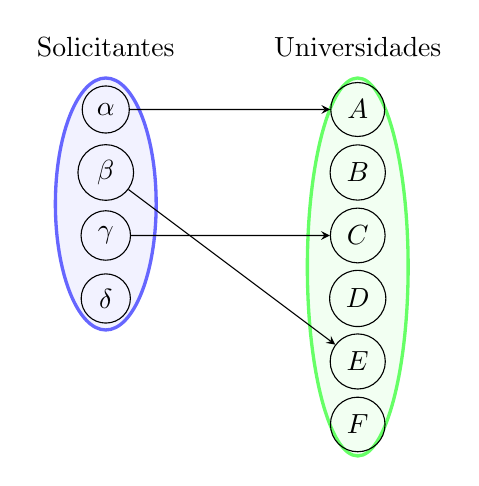
\begin{tikzpicture}[ scale=0.8]
\tikzset{vertex/.style = {shape=circle,draw,minimum size=1.5em}}
\tikzset{edge/.style = {->,> = latex}}
\filldraw[color=blue!60, fill=blue!5, very thick](0,2.5) ellipse (.8 and 2);
\filldraw[color=green!60, fill=green!5, very thick](4,1.5) ellipse (.8 and 3);


% vertices
% 


\node[vertex] (a) at (0,4) {$\alpha$};
\node[vertex] (b) at (0,3) {$\beta$};
\node[vertex] (c) at (0,2) {$\gamma$};
\node[vertex] (d) at (0,1) {$\delta$};


\node[vertex] (e) at (4,4) {$A$};
\node[vertex] (f) at (4,3) {$B$};
\node[vertex] (g) at (4,2) {$C$};
\node[vertex] (h) at (4,1) {$D$};
\node[vertex] (i) at (4,0) {$E$};
\node[vertex] (j) at (4,-1) {$F$};

\node (k) at (0,5) {Solicitantes};
\node (l) at (4,5) {Universidades};

\path[-stealth] (a) edge (e);
\path[-stealth] (b) edge (i);
\path[-stealth] (c) edge (g);
%\path[-stealth] (b) edge (g);

%\draw (4,4) node[cross=8pt,red] {};


%\draw (0.2,8)--(3.8,8);



\end{tikzpicture}

\end{figure}
\end{minipage}%
\begin{minipage}{.5\linewidth}
\begin{figure}[H]\centering

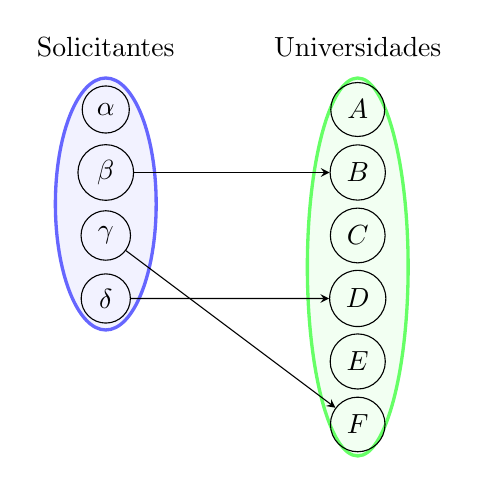
\begin{tikzpicture}[ scale=0.8]
\tikzset{vertex/.style = {shape=circle,draw,minimum size=1.5em}}
\tikzset{edge/.style = {->,> = latex}}
\filldraw[color=blue!60, fill=blue!5, very thick](0,2.5) ellipse (.8 and 2);
\filldraw[color=green!60, fill=green!5, very thick](4,1.5) ellipse (.8 and 3);


% vertices
% 


\node[vertex] (a) at (0,4) {$\alpha$};
\node[vertex] (b) at (0,3) {$\beta$};
\node[vertex] (c) at (0,2) {$\gamma$};
\node[vertex] (d) at (0,1) {$\delta$};


\node[vertex] (e) at (4,4) {$A$};
\node[vertex] (f) at (4,3) {$B$};
\node[vertex] (g) at (4,2) {$C$};
\node[vertex] (h) at (4,1) {$D$};
\node[vertex] (i) at (4,0) {$E$};
\node[vertex] (j) at (4,-1) {$F$};

\node (k) at (0,5) {Solicitantes};
\node (l) at (4,5) {Universidades};

\path[-stealth] (b) edge (f);
\path[-stealth] (c) edge (j);
\path[-stealth] (d) edge (h);
%\path[-stealth] (b) edge (g);

%\draw (4,4) node[cross=8pt,red] {};


%\draw (0.2,8)--(3.8,8);



\end{tikzpicture}
\end{figure}
\end{minipage}
\caption{Asignaciones estables.}
\end{figure}
\fin
\end{eje}

En lo que sigue de la tesis analizaremos una variante del problema con cotas comunes en el que las restricciones tienen la propiedad de ser anidadas. Veremos que este problema resulta mucho más sencillo de resolver y que además tiene propiedades bastante interesantes.





%\begin{eje}
%Contraejemplo de que no siempre existe usando \ref{listprefeje}
%\end{eje}


